% !TeX spellcheck = en_US 
\subsubsection*{Analysis}
\begin{tabular}{@{}l l}
\textbf{Scope}:&The AuctionHouse\textsuperscript{TM} automated administration system\\
\textbf{Level}:&User goal\\
\textbf{Primary Actor}:&Viewer\\
\textbf{Stakeholders and Interests}:&\begin{tabular}[t]{@{}l}Viewer: wants to make a reservation for a book in the catalogue.\end{tabular}\\
\textbf{Preconditions}:&\begin{tabular}[t]{@{}l}User is identified and authenticated.\end{tabular}\\
\textbf{Postconditions}:&\begin{tabular}[t]{@{}l}The selected book is marked in the system as reserved by the user and becomes\\ unavailable for other reservations. \\The user is notified of confirmation or failure of the reservation.\end{tabular}\\
\textbf{Frequency of occurence}:& \begin{tabular}[t]{@{}l}Difficult to estimate. Will correlate with the number of displayed books and \\the books themselves (their title, rarity etc.) for each particular opening day. \\Expected to be at least 2-3 reservations before each day when book stockroom opens, \\that is $\approx 2.5 \cdot 2 \cdot 4 = 20$ times per month.\end{tabular}
\end{tabular}\\\\
\textsl{Main Success Scenario}
\begin{enumerate}[noitemsep]
	\item The user requests the system to make a book reservation.
	\item The system presents all the books. 
	\item The user selects the desired book he wants to make a reservation for.
	\item The system checks if the selected book has been already reserved.
	\item If the selected book is already reserved, show "Failed" and the reason, else mark the book as being reserved by the user and show "Successful".
\end{enumerate}
\textsl{Extensions}
\begin{itemize}[noitemsep]
	\item When the user has a greater number of book reservations than the admissible number, the system shows "You reached the maximum number of book reservations" and denies the user access to making a new reservation.
\end{itemize}
\textsl{System Sequence Diagram}
\begin{figure}[H]
	\centering
	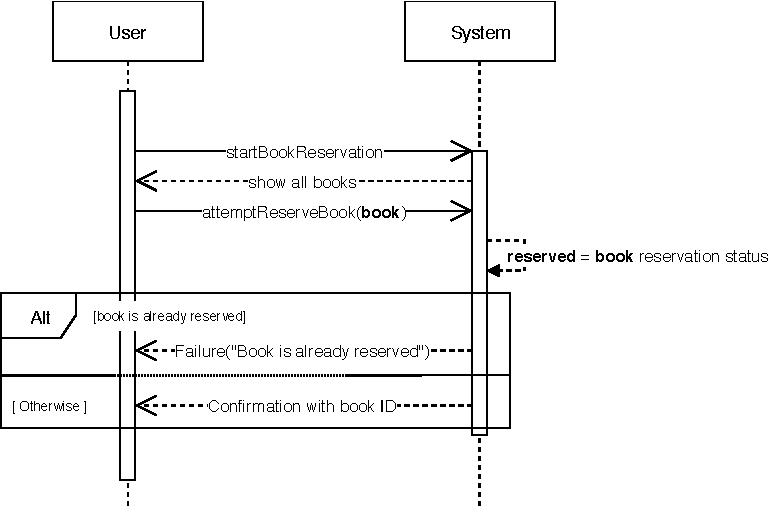
\includegraphics[scale=1]{uml/SD-bb-reserve.pdf}
	\caption*{Interactions displayed in a System Sequence Diagram defined by the MSS and its extensions in blackbox format}
\end{figure}